\documentclass[
  a4paper,
  spanish,
  12pt,
]{scrartcl}

\linespread{1.05}
%\setlength{\parindent}{18pt}


%-------------------------------------------------------------------------------
%	PAQUETES
%-------------------------------------------------------------------------------

% Idioma

\usepackage{indentfirst}
% Matemáticas

\usepackage{mathrsfs}

\usepackage{config}
\usepackage{amsmath, amsthm, amssymb}
% \usepackage{mathtools}
% \usepackage{commath}
% \usepackage{xfrac}
\usepackage{graphicx}



% Fuentes personalizadas para utilizar con XeLaTeX o LuaLaTeX

\usepackage[no-math]{fontspec}
\setmainfont[WordSpace=1.3, RawFeature={+ss06}]{EBGaramond}
\setsansfont[Scale=0.9]{Alegreya Sans}
\setmonofont[Scale=0.75]{Bitstream Vera Sans Mono}

\usepackage[math-style=TeX]{unicode-math}
\setmathfont{Garamond Math}[StylisticSet={3}]


% Configuración de microtype

\defaultfontfeatures{Ligatures=TeX,Numbers=Lining}
\usepackage[activate={true,nocompatibility},final,tracking=true,factor=1100,stretch=10,shrink=10]{microtype}
\SetTracking{encoding={*}, shape=sc}{0}

% Enlaces y colores

\usepackage{hyperref}
\usepackage{xcolor}
\hypersetup{
  colorlinks=true,
  citecolor=,
  linkcolor=,
  urlcolor=blue,
}

% Otros elementos de página

\usepackage{enumitem}
\setlist[enumerate]{leftmargin=-\itemindent, itemsep=0pt}
\setlist[itemize]{leftmargin=-\itemindent, itemsep=0pt}
%\setlist[itemize]{leftmargin=*}
%\setlist[enumerate]{leftmargin=*}

\usepackage[labelfont={sc, sf}, textfont=sf]{caption}

\usepackage{booktabs}
\renewcommand\arraystretch{1.5}

% Tikz

\usepackage{tikz}
\usetikzlibrary{babel}
\usepackage{float}

% Código

\usepackage{listings}
\lstset{
	basicstyle=\ttfamily,%
	breaklines=true,%
	captionpos=b,                    % sets the caption-position to bottom
  tabsize=2,	                   % sets default tabsize to 2 spaces
  frame=lines,
  numbers=left,
  stepnumber=1,
  aboveskip=12pt,
  showstringspaces=false,
  keywordstyle=\bfseries,
  commentstyle=\itshape,
  columns=flexible,
}
\renewcommand{\lstlistingname}{Listado}

% ENTORNOS

\usepackage[theorems, skins, breakable]{tcolorbox}

\tcolorboxenvironment{nth}{
	blanker,
	breakable,
	left=12pt,
	before skip=12pt,
	after skip=12pt,
	borderline west={2pt}{0pt}{500},
	before upper={\parindent 12pt},
}

\tcolorboxenvironment{nprop}{
	blanker,
	breakable,
	left=12pt,
	before skip=12pt,
	after skip=12pt,
	borderline west={2pt}{0pt}{42},
	before upper={\parindent 12pt},
}

\tcolorboxenvironment{ncor}{
	blanker,
	breakable,
	left=12pt,
	before skip=12pt,
	after skip=12pt,
	borderline west={2pt}{0pt}{300},
	before upper={\parindent 12pt},
}

\tcolorboxenvironment{ndef}{
	skin=enhancedmiddle jigsaw,
	frame hidden,
	colback= 36,
	breakable = true,
	break at = -6pt,
	top = 4pt,       % Estos márgenes están un poco a ojo
	bottom = 4pt,
	left= 8pt,
	right = 8pt,
	before skip=8pt, % Normalmente dejamos 12pt, pero
	after skip=8pt,  % aquí tenemos espacio adicional por el fondo
	no borderline,
	borderline west={2pt}{0pt}{42},
	before upper={\parindent 12pt},
}

\tcolorboxenvironment{ejer}{
	skin=enhancedmiddle jigsaw,
	frame hidden,
	colback=50,
	breakable = true,
	break at = -6pt,
	top = 4pt,       % Estos márgenes están un poco a ojo
	bottom = 4pt,
	left= 8pt,
	right = 8pt,
	before skip=8pt, % Normalmente dejamos 12pt, pero
	after skip=8pt,  % aquí tenemos espacio adicional por el fondo
	no borderline,
	borderline west={2pt}{0pt}{500},
	borderline east={2pt}{0pt}{50},
	before upper={\parindent 12pt},
}


% Márgenes
\usepackage[bottom=3.125cm, top=2.5cm, left=3.5cm, right=3.5cm, marginparwidth=70pt]{geometry}

%dealing with (sub/subsub)sections
%\let\raggedsection\centering%Center all sectioningheads
%all levels have something in common, let's save typing:
\RedeclareSectionCommands[beforeskip=-3ex,
afterskip=2ex]{section,subsection,subsubsection}
\addtokomafont{section}{\normalfont\large\textsc}
\RedeclareSectionCommand[beforeskip=-6ex]{section}
\addtokomafont{subsection}{\normalfont\itshape}

%-------------------------------------------------------------------------------
%	CONTENIDO
%-------------------------------------------------------------------------------

\begin{document}

\begin{flushright}
  Ricardo Ruiz Fernández de Alba\vspace{.5em}

  \textit{Topología II}

  Doble Grado en Ingeniería Informática y Matemáticas

  \textsc{Universidad de Granada}\vspace{.5em}

  \today\vspace{.5em}
\end{flushright}

\begin{flushleft}
  \scshape\Large Relación de Ejercicios del Tema 1
\end{flushleft}


\begin{ejer}
(1) Dado un grupo $G$, se define el centro de $G$ como

$$
Z(G)=\{x \in G / x \cdot y=y \cdot x, \forall y \in G\} .
$$

Demostrar que $Z(G)$ es un subgrupo de $G$, y que $G$ es abeliano si y sólo si $Z(G)=G$.\\
\end{ejer}

\begin{sol}

Sea $x, y \in Z(G)$. Sea $w \in G$, entonces $yw = wy$ y $w^{-1}y^{-1} = y^{-1}w^{-1}$, luego $y^{-1} \in Z(G)$.
Sea ahora $z \in G$. Se tendrá que $xy^{-1}z = xzy^{-1} = zxy^{-1}$, donde se ha utilizado que $x,y^{-1} \in Z(G)$.
Así, $Z(G) \leq G$.

$G$ es es abeliano si cada elemento conmuta con todos los demas,
equivalentemente su centro (subconjunto de elementos que conmutan con todos) es todo $G$ 
(todos conmutan).

\end{sol}

\begin{ejer}
(2) Probar que son grupos topológicos:\\
(a) $\mathbb{R}^{n}$ con la suma y la topología usuales.\\
(b) $\mathbb{R}_{*}=\mathbb{R} \backslash\{0\}$ y $\mathbb{C}_{*}=\mathbb{C} \backslash\{0\}$ con los productos y las topologías usuales.\\
(c) $\mathbb{S}^{1} \subset \mathbb{C}$ con el producto de números complejos y la topología usual.\\
(d) El grupo lineal general $GL(n)$, el grupo ortogonal $\mathrm{O}(n)$ y el grupo especial ortogonal $\mathrm{SO}(n)$ con el producto de matrices y la topología inducida por $M_{n}(\mathbb{R}) \equiv \mathbb{R}^{n^{2}}$.\\
\end{ejer}

\begin{sol}

(a)

\begin{itemize}
\item{$(\mathbb{R}^n, +)$ es un grupo algebraico.}
\item{$(\mathbb{R}^n, \tau_u)$ un espacio topológico.}
\item{La aplicación $\Phi: \mathbb{R}^n \times \mathbb{R}^N \rightarrow \mathbb{R}^n$ dada por

$\Phi(x_1, x_2) = x_1 - x_2$ es continua}
\end{itemize}

(b)

\begin{itemize}
\item{$(\mathbb{R_*}, \cdot)$ y $(\mathbb{C_*}, \cdot)$ son grupos algebraicos.}
\item{$(\mathbb{R_*}, \tau_u)$ y $(\mathbb{C_*}, \tau_u)$ son espacios topológicos.}
\item{La aplicación $\Phi_1: R_* \times R_* \rightarrow G$  y la 
aplicación $\Phi_2: C_* \times C_* \rightarrow G$ dadas por
	
$\Phi_1(x_1, x_2) = x_1 \cdot x_2^{-1}$ es continua con $x_1, x_2 \in \mathbb{R} \setminus \{0\}$ \\
$\Phi_2(x_1, x_2) = x_1 \cdot x_2^{-1}$ es continua con $x_1, x_2 \in \mathbb{C} \setminus \{0\}$.}
\end{itemize}

(c)


\begin{itemize}
\item{$(\mathbb{S^1}, \cdot)$ es un grupo algebraico. Pues dado $z=e^{2\pi it}$, se tiene que $z^{-1}=e^{-2\pi it} \in \mathbb{S}^1$}
\item{$(\mathbb{S^1}, \tau_u)$ es un espacio topológico (con la topología inducida)}
\item{La aplicación $\Phi: \mathbb{S}^1 \times \mathbb{S}^1 \rightarrow G$  
	
$\Phi_1(z_1, z_2) = z_1 \cdot z_2^{-1}$ es continua con $z_1, z_2 \in \mathbb{S}^1$ \\
}
\end{itemize}

(d) 

\begin{itemize}
\item{$GL(n)$ es un grupo algebraico pues toda matriz cuadrada regular tiene inversa.}
\item{Considerando la topología inducida por $\mathbb{R}^{n^2}$, es además un espacio topológico.}
\item{La aplicación $\Phi: GL(n) \times GL(n) \rightarrow GL(n)$ dada por $\Phi(A, B) = AB^{-1}$
es continua matricialmente (fórmula de la inversa , cofactores y determinante y producto de matrices continuo)}
\end{itemize}

\begin{itemize}
\item{$O(n)$ es un grupo algebraico pues toda matriz cuadrada ortogonal tiene inversa, que coincide con su traspuesta.}
\item{Considerando la topología inducida por $\mathbb{R}^{n^2}$, es además un espacio topológico.}
\item{La aplicación $\Phi: O(n) \times O(n) \rightarrow O(n)$ dada por $\Phi(A, B) = AB^{-1}$
es continua matricialmente (fórmula de la inversa , cofactores y determinante y producto de matrices continuo)}
\end{itemize}

\begin{itemize}
\item{$SO(n)$ es un grupo algebraico pues toda matriz cuadradaa con determinante 1 tiene inversa.}
\item{Considerando la topología inducida por $\mathbb{R}^{n^2}$, es además un espacio topológico.}
\item{La aplicación $\Phi: SO(n) \times SO(n) \rightarrow SO(n)$ dada por $\Phi(A, B) = AB^{-1}$
es continua matricialmente (fórmula de la inversa , cofactores y determinante y producto de matrices continuo)}
\end{itemize}

\end{sol}

\begin{ejer}
(3) Sean $f, g:[0,1] \rightarrow X$ arcos con el mismo punto inicial $x \in X$ y el mismo punto final $y \in Y$. Demostrar que $f \simeq g$ si solo si $f * \bar{g}$ es un lazo homotópico al lazo constante $\varepsilon_{x}$.\\
\end{ejer}


\begin{sol}

Usaremos las siguientes propiedades:

Si $f \simeq g$, entonces $f*h \simeq g*h$, empezando $h$ en $z$ y acabando en $x$. 
Además $g * \bar{g} \simeq \varepsilon_x$.

\newpage 

$\boxed{\Rightarrow}\;\;$ Considerando $h = \bar{g}$, tenemos que $f*\bar{g} \simeq g * \bar{g} \simeq \varepsilon_x$. 

$\boxed{\Leftarrow}\;\;$ Considerando $h = g$, tenemos que si $f * \bar{g} \simeq \varepsilon_x $ entonces 

$$f * \bar{g} * g \simeq \varepsilon_x * g$$
$$f * \varepsilon_x \simeq \varepsilon_x * g$$
$$f \simeq g$$


\end{sol}


\begin{ejer}
(4) Demostrar que si $f, g:[0,1] \rightarrow X$ son arcos con $f(1)=g(0)$ entonces $\overline{f * g}=\bar{g} * \bar{f}$\\
\end{ejer}

$$
\overline{(f*g)}(t) = (f*g)(1-t) =
\begin{cases} 
    f(2 - 2t) & \text{si } t \in \left( \frac{1}{2}, 1 \right], \\
    g(2(1 - t) - 1) & \text{si } t \in \left( 0, \frac{1}{2} \right]
\end{cases} =
$$
$$
= \begin{cases} 
    g(1 - 2t) & \text{si } t \in \left( 0, \frac{1}{2} \right],  \\
    f(2 - 2t) & \text{si } t \in \left( \frac{1}{2}, 1 \right]
\end{cases}
$$

$$
(\bar{g}*\bar{t})(t) = 
\begin{cases} 
    \bar{g}(2t) & \text{si } t \in \left( 0, \frac{1}{2} \right], \\
    \bar{f}(2t-1) & \text{si } t \in \left( \frac{1}{2}, 1 \right]
\end{cases} =
$$

$$
= \begin{cases} 
    g(1-2t) & \text{si } t \in \left( 0, \frac{1}{2} \right], \\
    f(1-2t+1) & \text{si } t \in \left( \frac{1}{2}, 1 \right]
\end{cases} =
\begin{cases} 
    g(1-2t) & \text{si } t \in \left( 0, \frac{1}{2} \right], \\
    f(2-2t) & \text{si } t \in \left( \frac{1}{2}, 1 \right]
\end{cases}
$$

\begin{ejer}
(5) Sea $f: X \rightarrow Y$ una aplicación continua entre espacios topológicos. Tomamos dos puntos $x_{1}$ y $x_{2}$ en $X$. Denotamos por $\left(f_{*}\right)_{1}: \Pi_{1}\left(X, x_{1}\right) \rightarrow \Pi_{1}\left(Y, f\left(x_{1}\right)\right)$ y por $\left(f_{*}\right)_{2}: \Pi_{1}\left(X, x_{2}\right) \rightarrow \Pi_{1}\left(Y, f\left(x_{2}\right)\right)$ a los homomorfismos inducidos por $f$ en los puntos $x_{1}$ y $x_{2}$. Sea $\gamma:[0,1] \rightarrow X$ un arco con $\gamma(0)=x_{1} \mathrm{y}$ $\gamma(1)=x_{2}$. Demostrar que

$$
\left(f_{*}\right)_{2} \circ F_{\gamma}=F_{f \circ \gamma} \circ\left(f_{*}\right)_{1},
$$

donde $F_{\gamma}: \Pi_{1}\left(X, x_{1}\right) \rightarrow \Pi_{1}\left(X, x_{2}\right)$ es el isomorfismo inducido por $\gamma$ y $F_{f \circ \gamma}: \Pi_{1}\left(Y, f\left(x_{1}\right)\right) \rightarrow$ $\Pi_{1}\left(Y, f\left(x_{2}\right)\right)$ es el inducido por el arco $f \circ \gamma:[0,1] \rightarrow Y$.\\
\end{ejer}

\begin{ejer}
(6) (Grupo fundamental de un producto). Sean $X$ e $Y$ dos espacios con puntos base $x_{0} \in X$ e $y_{0} \in Y$. Sea $\Phi: \Pi_{1}\left(X, x_{0}\right) \times \Pi_{1}\left(Y, y_{0}\right) \rightarrow \Pi_{1}\left(X \times Y,\left(x_{0}, y_{0}\right)\right)$ dada por:


$$
\Phi([\alpha],[\beta])=[(\alpha, \beta)]
$$

donde $(\alpha, \beta):[0,1] \rightarrow X \times Y$ es el arco $(\alpha, \beta)(t)=(\alpha(t), \beta(t))$. Demostrar que $\Phi$ está bien definida y es un isomorfismo. Concluir que:

$$
\Pi_{1}\left(X \times Y,\left(x_{0}, y_{0}\right)\right) \cong \Pi_{1}\left(X, x_{0}\right) \times \Pi_{1}\left(Y, y_{0}\right)
$$
\end{ejer}


\begin{ejer}
(7) Sean $X$ un espacio topológico y $x \in X$ un punto.\\
(a) Sea $\gamma:[0,1] \rightarrow X$ un lazo con base $x$. Demostrar que el isomorfismo $F_{\gamma}: \Pi_{1}(X, x) \rightarrow \Pi_{1}(X, x)$ es la identidad si y solo si la clase de homotopía $[\gamma]$ pertenece al centro de $\Pi_{1}(X, x)$ (ver ejercicio (1) para la definición de centro de un grupo).\\
(b) Sean $\gamma, \mu:[0,1] \rightarrow X$ arcos con punto inicial $x \in X$ y punto final $y \in X$. Encontrar una condición necesaria y suficiente para que los isomorfismos $F_{\gamma}, F_{\mu}: \Pi_{1}(X, x) \rightarrow \Pi_{1}(X, y)$ sean iguales.\\
\end{ejer}

\begin{ejer}
(8) Demostrar que toda aplicación continua $f: \mathbb{S}^{1} \rightarrow \mathbb{S}^{1}$ admite una extensión continua $F: \overline{\mathbb{D}} \rightarrow \overline{\mathbb{D}}$, donde $\overline{\mathbb{D}}=\left\{(x, y) \in \mathbb{R}^{2}: x^{2}+y^{2} \leq 1\right\}$ es el disco unidad cerrado.\\
\end{ejer}

\begin{figure}[h]
    \centering
    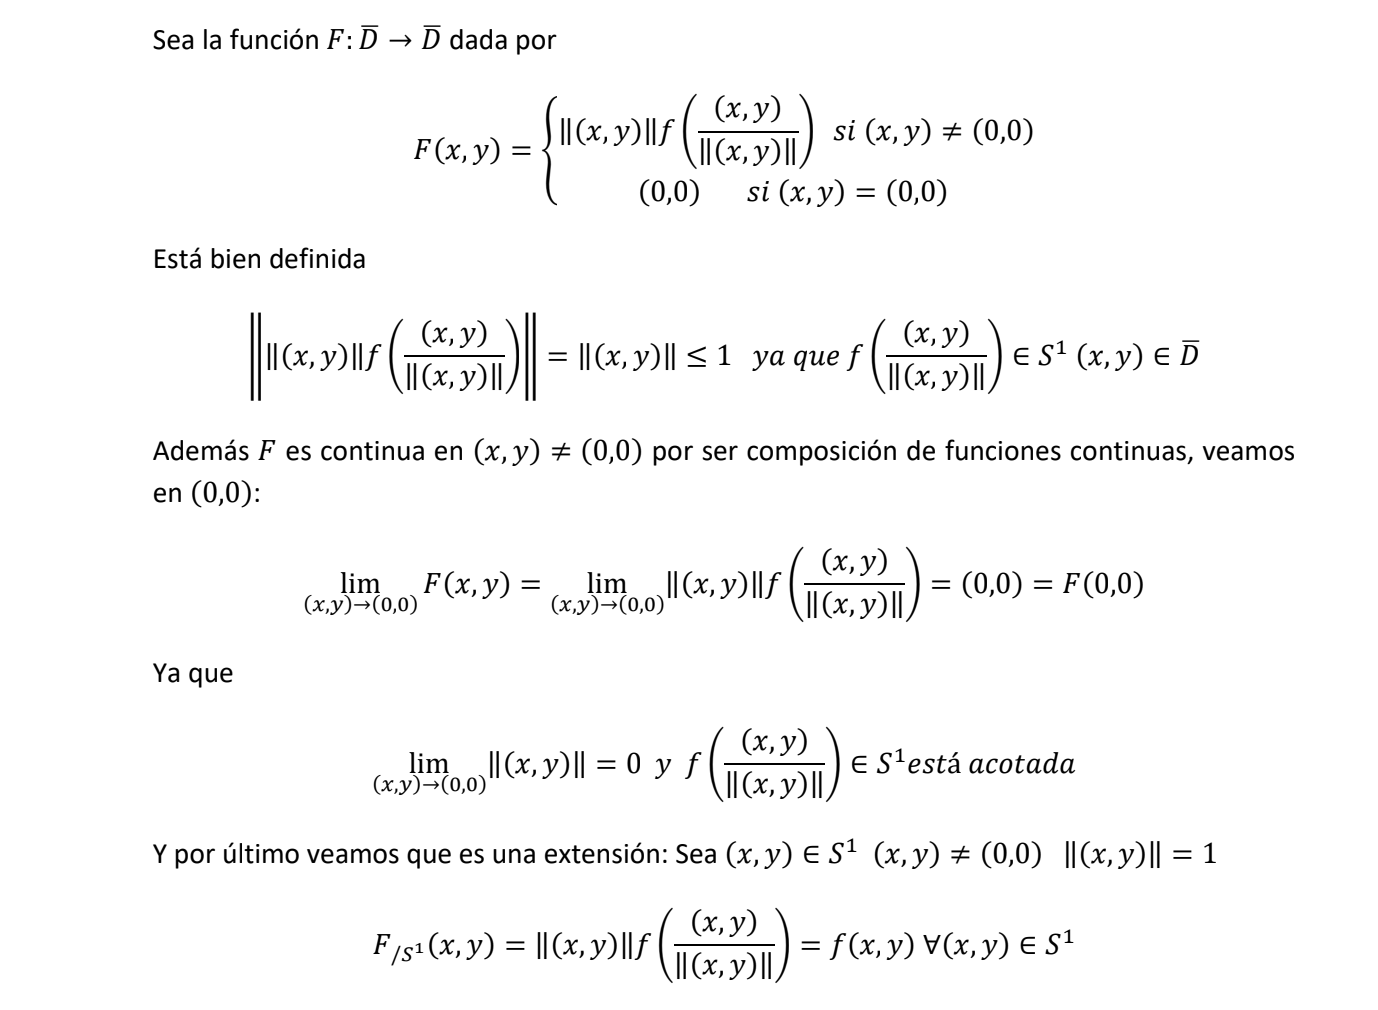
\includegraphics[width=\textwidth]{ej8.png}
    \label{fig:etiqueta}
\end{figure}


\begin{ejer}
(9) Sea $f \in \Omega_{1}\left(\mathbb{S}^{1}\right)$ un lazo de clase $C^{1}$. Demostrar que:

$$
\operatorname{deg}(f)=\frac{1}{2 \pi} \int_{0}^{1}\left\langle f^{\prime}(u), J(f(u))\right\rangle d u
$$

donde $J: \mathbb{R}^{2} \rightarrow \mathbb{R}^{2}$ es el giro de ángulo $\pi / 2$ dado por $J(x, y)=(-y, x)$.\\
\end{ejer}

\begin{ejer}
(10) (Conjuntos estrellados). Sea $X \subseteq \mathbb{R}^{n}$ y $x_{0} \in X$. Se dice que $X$ es estrellado respecto de $x_{0}$ si el segmento $\left[x_{0}, x\right] \subseteq X$ para cada $x \in X$.\\
(a) Sean $f, g \in \Omega_{x_{0}}(X)$ lazos en $X$ con base $x_{0}$. Demostrar que $f \simeq g$ y construir una homotopía de $f$ a $g$ en $X$ de forma explícita. Concluir que $X$ es simplemente conexo.\\
(b) Sean $F, G: Y \rightarrow X$ dos aplicaciones continuas donde $Y$ es cualquier espacio topológico. Demostrar que $F \simeq G$.\\
\end{ejer}

\begin{ejer}
(11) Sean $f, g: \mathbb{R}^{2} \rightarrow \mathbb{R}^{2}$ aplicaciones continuas y acotadas. Demostrar que existe un punto $q \in \mathbb{R}^{2}$ tal que $f(q)=q-3 g(q)$.\\
\end{ejer}

\begin{sol}
Como están acotadas, $\operatorname{Im} f \subset \bar{B}(0, R)$ y $\operatorname{Im} g \subset \bar{B}(0, R')$ para ciertos $R < R' \in \mathbb{R}$.
Así, $f : \mathbb{R}^2 \rightarrow \bar{B}(0, R)$ y $g: \mathbb{R}^2 \rightarrow \bar{B}(0, R)$
serán continuas y sobreyectivas y podemos restringir el dominio, conservando la continuidad:

$$
f: \bar{B}(0, R) \rightarrow \bar{B}(0, R)
$$

$$
g: \bar{B}(0, R) \rightarrow \bar{B}(0, R)
$$

Sea $h: \bar{B}(0,R) \rightarrow \bar{B}(0, R)$ dada por
$$ h(x) = f(x) + 3g(x) $$

Es continua por ser suma de continuas. Utilizando que $\bar{B}(0, R) \cong \bar{D}$
y el Ejercicio variación del Teorema del Punto Fijo de Brouwer, obtenemos que $\exists q \in \bar{B}(0, R) $ tal que
$h(q) = q$.

Luego $f(q) + 3g(q) = q$ y $f(q) = q - 3g(q)$, como ser quería.

\end{sol}

\begin{ejer}
(12) Demostrar que el sistema de ecuaciones

$$
\left\{\begin{aligned}
x-\operatorname{arctg}\left(x^{2}-y^{3}\right) & =5, \\
\cos (x)+\operatorname{sen}\left(x y^{3}\right)+e^{x}+e^{y^{2}}+\frac{1}{y} & =-3 .
\end{aligned}\right.
$$

tiene al menos una solución $(x, y)$ en $\mathbb{R}^{2}$.\\
\end{ejer}

\begin{figure}[h]
	\centering
	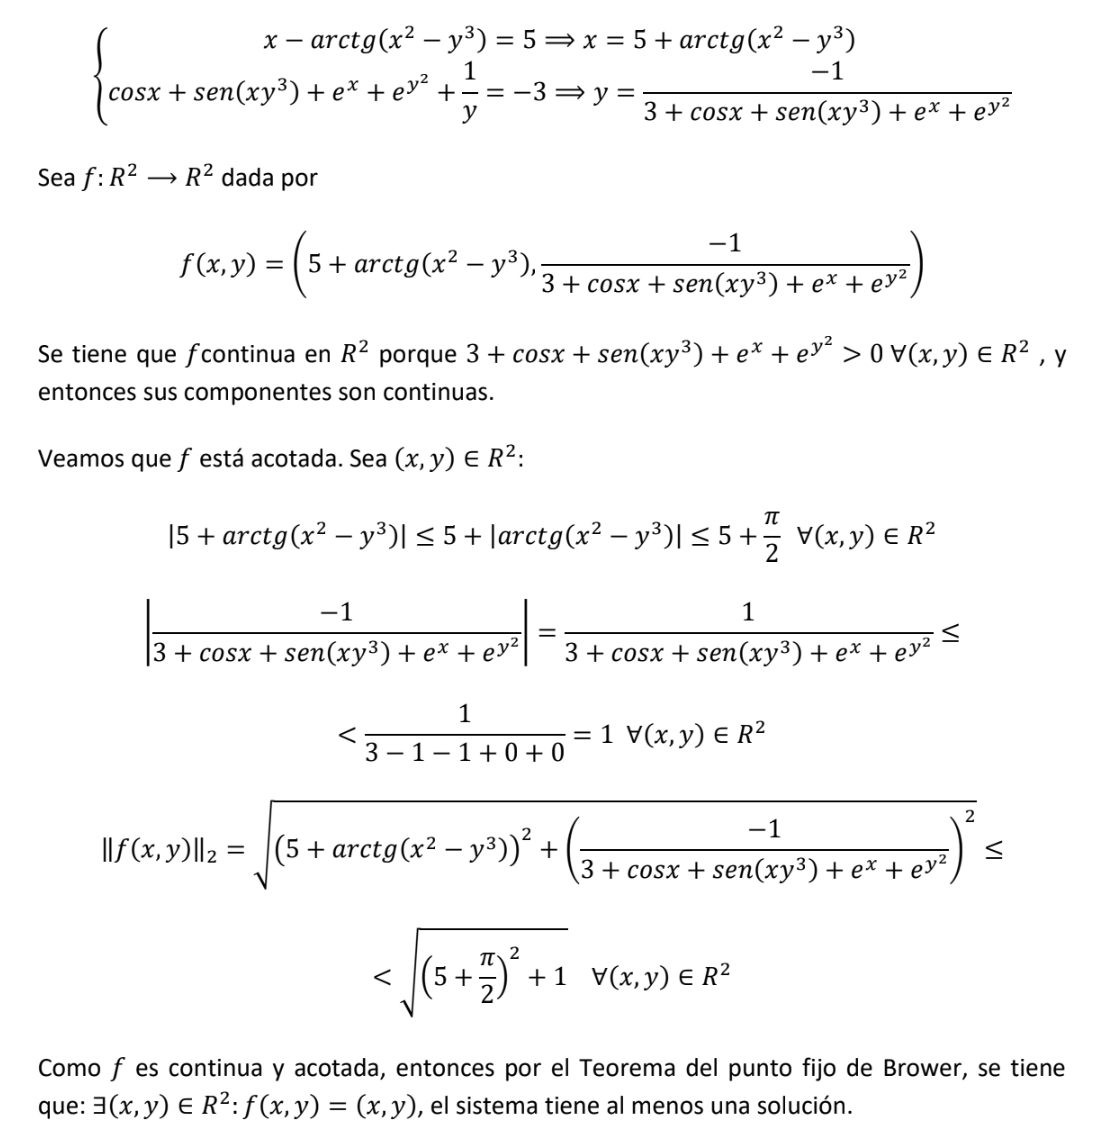
\includegraphics[width=\textwidth]{ej12.png}
\end{figure}

\newpage

\begin{ejer}
(13) Sean $X$ un espacio topológico y $F, G: X \rightarrow \mathbb{S}^{n}$ aplicaciones continuas con $G(x) \neq-F(x)$ para todo $x \in X$. Demostrar que $F \simeq G$. Deducir que:\\
(a) Si $F: \mathbb{S}^{n} \rightarrow \mathbb{S}^{n}$ es continua y no tiene puntos fijos, entonces $F \simeq-\operatorname{Id}_{\mathbb{S}^{n}}$.\\
(b) Si $F: \mathbb{S}^{n} \rightarrow \mathbb{S}^{n}$ es continua y $F(x) \neq-x$ para todo $x \in \mathbb{S}^{n}$, entonces $F \simeq \operatorname{Id}_{\mathbb{S}^{n}}$.\\
\end{ejer}

\begin{ejer}
(14) Demostrar que $\mathrm{Id}_{\mathbb{S}^{2 n-1}} \simeq-\mathrm{Id}_{\mathbb{S}^{2 n-1}}$ para todo $n \in \mathbb{N}$. A partir de este hecho y del ejercicio anterior deducir que si $f: \mathbb{S}^{1} \rightarrow \mathbb{S}^{1}$ es continua y homotópica a una función constante, entonces existen $x_{1}, x_{2} \in \mathbb{S}^{1}$ tales que $f\left(x_{1}\right)=x_{1}$ y $f\left(x_{2}\right)=-x_{2}$.\\
\end{ejer}

\begin{ejer}
(15) Demostrar que para todo espacio topológico $X$ la sección ecuatorial $A=X \times\{0\}$ es un retracto de deformación de $X \times[-1,1]$. Deducir el tipo de homotopía de la banda $\mathbb{R}^{n} \times[-1,1]$, el cilindro $\mathbb{S}^{n} \times[-1,1]$ y el cubo $[-1,1]^{n+1}$. Discutir qué ocurre si sustituimos $[-1,1]$ por $\mathbb{R}$.\\
\end{ejer}

\begin{ejer}
(16) Encontrar un retracto de deformación de $X=\mathbb{S}^{n} \backslash\{N, S\}$ y otro de $X=\mathbb{R}^{n+1} \backslash \overline{\mathbb{B}}(0,1)$, donde $\overline{\mathbb{B}}(0,1)$ es la bola unidad cerrada.\\
\end{ejer}

\begin{ejer}
(17) Sean $x_{1}, x_{2} \in \mathbb{R}^{2} \operatorname{con} x_{1} \neq x_{2}$. Definimos $A=C_{1} \cup C_{2}$, donde $C_{i}$ es la circunferencia de centro $x_{i}$ y radio $\left\|x_{1}-x_{2}\right\| / 2$. Demostrar gráficamente que $A$ es un retracto de deformación de $\mathbb{R}^{2} \backslash\left\{x_{1}, x_{2}\right\}$. Calcular explícitamente la retracción cuando $x_{1}=(-1,0)$ y $x_{2}=(1,0)$.\\
\end{ejer}

\begin{ejer}
(18) ¿Es cierto el teorema de Borsuk-Ulam si cambiamos $\mathbb{S}^{2}$ por el toro $T=\mathbb{S}^{1} \times \mathbb{S}^{1}$ ?\\
\end{ejer}

\begin{ejer}
(19) Probar que el teorema de Borsuk-Ulam es equivalente a cualquiera de los siguientes enunciados:\\
(a) Si $f: \mathbb{S}^{2} \rightarrow \mathbb{R}^{2}$ es continua e impar, entonces existe $x_{0} \in \mathbb{S}^{2}$ tal que $f\left(x_{0}\right)=0$.\\
(b) Si $g_{1}, g_{2}: \mathbb{S}^{2} \rightarrow \mathbb{R}$ son continuas e impares, existe $x_{0} \in \mathbb{S}^{2}$ tal que $g_{1}\left(x_{0}\right)=g_{2}\left(x_{0}\right)=0$.\\
\end{ejer}

\begin{ejer}
(20) Sea $f: \overline{\mathbb{D}} \rightarrow \overline{\mathbb{D}}$ un homeomorfismo. Demostrar que $f$ conserva el interior y la frontera de $\overline{\mathbb{D}}$.\\
\end{ejer}

\begin{ejer}
(21) Sea $\left.f: \mathbb{R} \rightarrow \mathbb{R}^{+}=\right] 0,+\infty[$ una función continua y sea

$$
S_{f}=\left\{(x, y, z) \in \mathbb{R}^{3}: x^{2}+y^{2}=f(z)^{2}\right\}
$$

(a) Estudiar el conjunto $S_{f} \cap\left\{z=z_{0}\right\}$ con $z_{0} \in \mathbb{R}$. Esbozar un dibujo de $S_{f}$.\\
(b) Demostrar que si $g: \mathbb{R} \rightarrow \mathbb{R}^{+}$es otra función continua entonces $S_{g}$ es homeomorfo a $S_{f}$.\\
(c) Calcular el grupo fundamental de $S_{f}$.\\

\end{ejer}

\begin{ejer}
(22) Encontrar un retracto de deformación de $\mathbb{R}^{3} \backslash L$, donde $L=\left\{(x, y, z) \in \mathbb{R}^{3}: x=y=0\right\}$ es el eje $z$. Obtener $\Pi_{1}\left(\mathbb{R}^{3} \backslash R\right)$, siendo $R$ cualquier recta afín en $\mathbb{R}^{3}$ (intenta utilizar que hay una retracción de $\mathbb{R}^{2} \backslash\{0\}$ en $\left.\mathbb{S}^{1}\right)$.\\
\end{ejer}

\begin{ejer}
(23) Sea $S$ un subespacio afín de dimensión $k \leq n-2$ en $\mathbb{R}^{n}$. Calcular $\Pi_{1}\left(\mathbb{R}^{n} \backslash S\right)$ encontrando para ello un retracto de deformación.\\
\end{ejer}

\begin{ejer}
(24) Demostrar que un abierto de $\mathbb{R}^{2}$ no puede ser homeomorfo a un abierto de $\mathbb{R}^{n}$ si $n \neq 2$.\\
\end{ejer}

\begin{ejer}
(25) Sea $A$ un retracto de un disco cerrado en $\mathbb{R}^{2}$. Demostrar que toda aplicación continua $f: A \rightarrow A$ tiene al menos un punto fijo. Deducir que toda aplicación continua $f: X \rightarrow X$ con $X=\overline{\mathbb{B}}((-1,0), 1) \cup$ $\overline{\mathbb{B}}((1,0), 1)$ tiene al menos un punto fijo.\\
\end{ejer}

\begin{ejer}
(26) Calcular $\Pi_{1}(X)$ en estos casos:\\
(a) $X=\mathbb{S}^{2} \cup[N, S]$, donde $N$ y $S$ son el polo Norte y el polo Sur de $\mathbb{S}^{2}$.\\
(b) $X=\mathbb{S}^{2} \cup\left\{(x, y, 0) \in \mathbb{R}^{3}: x^{2}+y^{2} \leq 1\right\}$.\\
(c) $X=\mathbb{S}^{2} \cup C_{1} \cup C_{2}$, donde $C_{1}$ y $C_{2}$ son circunferencias tangentes a $\mathbb{S}^{2}$ en los puntos $N$ y $S$, respectivamente.\\
(d) $X$ es la unión de una esfera y de un toro tangentes en un único punto.\\
(e) $X$ es la unión de dos toros tangentes en un único punto.\\
(f) $X$ es una botella de Klein.\\
\end{ejer}

\begin{ejer}
(27) Sea $X$ el espacio obtenido a partir de una corona circular plana cuando se identifican puntos antípodas en las dos circunferencias del borde. Calcular $\Pi_{1}(X)$.\\
\end{ejer}

\begin{ejer}
(28) Sea $f: A \rightarrow Y$ una aplicación continua con $A \subseteq X$ y $X$ simplemente conexo. Supongamos que existe $F: X \rightarrow Y$ continua con $F_{\mid A}=f$. Probar que el homomorfismo inducido $f_{*}: \Pi_{1}\left(A, x_{0}\right) \rightarrow \Pi_{1}\left(Y, f\left(x_{0}\right)\right)$ es trivial para todo $x_{0} \in A$.\\
\end{ejer}

\begin{ejer}
(29) Sean $f, g: X \rightarrow Y$ aplicaciones continuas con $f\left(x_{0}\right)=g\left(x_{0}\right)=y_{0}$. Supongamos que $f \simeq g$ por una homotopía $H: X \times[0,1] \rightarrow Y$ tal que $H\left(x_{0}, s\right)=y_{0}$ para todo $s \in[0,1]$. Demostrar que los homomorfismos inducidos $f_{*}$ y $g_{*}$ en $x_{0}$ son iguales.\\
\end{ejer}

\begin{ejer}
(30) Discutir si la bola unidad cerrada es un retracto de deformación de $\mathbb{R}^{n+1}$.\\
\end{ejer}

\begin{ejer}
(31) Sea $X$ simplemente conexo y $A \subseteq X$ un retracto de $X$. ¿Es $A$ simplemente conexo?\\
\end{ejer}

\begin{ejer}
(32) Sea $X \subset \mathbb{R}^{n}$ un convexo compacto con interior no vacío. Dado un punto $x_{0}$ del interior de $X$, demostrar que la frontera $\operatorname{Fr}(X)$ es un retracto de deformación de $X \backslash\left\{x_{0}\right\}$.\\
\end{ejer}

\begin{ejer}
(33) Discutir si $\mathbb{S}^{1}$ admite algún retracto de deformación $A \neq \mathbb{S}^{1}$.\\
\end{ejer}

\begin{ejer}
(34) Sea $f: \mathbb{S}^{1} \rightarrow \mathbb{S}^{1}$ la aplicación dada por $f(z)=z^{n}, n \in \mathbb{N}$. Calcular el homomorfismo inducido $f_{*}: \Pi_{1}\left(\mathbb{S}^{1}, 1\right) \rightarrow \Pi_{1}\left(\mathbb{S}^{1}, 1\right)$.\\
\end{ejer}

\begin{ejer}
(35) Sean $X$ un espacio topológico, $A \subseteq X$ un subconjunto y $a \in A$. ¿Es $\left(i_{A}\right)_{*}: \Pi_{1}(A, a) \rightarrow \Pi_{1}(X, a)$ un monomorfismo? ¿Y si $A$ es un retracto de $X$ ?\\
\end{ejer}

\begin{ejer}
(36) Supongamos que $f: X \rightarrow Y$ es continua y sobreyectiva con $f\left(x_{0}\right)=y_{0}$. ¿Es cierto que $f_{*}: \Pi_{1}\left(X, x_{0}\right) \rightarrow$ $\Pi_{1}\left(Y, y_{0}\right)$ es un epimorfismo?\\
\end{ejer}

\begin{ejer}
(37) ¿Es todo retracto de un espacio $X$ un retracto de deformación de $X$ ?\\
\end{ejer}

\begin{ejer}
(38) ¿Es cierto el teorema del punto fijo de Brouwer para $X=\mathbb{R}^{n}$ ? ¿Y para una corona?\\
\end{ejer}

\begin{ejer}
(39) Discutir si existe algún homeomorfismo de $\mathbb{R}^{2}$ que intercambie las dos componentes conexas de $\mathbb{R}^{2} \backslash \mathbb{S}^{1}$.
\end{ejer}


\end{document}
